\begin{lemma}
Tangent to a circle : Consider a circle 
\begin{align}
    \vec{x}^\top\vec{x} + 2\vec{c}^\top\vec{x} + f = 0 
\end{align}
Given a point $\vec{q}$ on the circle, the tangent at that point is given as,
\begin{align}
    \brak{\vec{q}+\vec{c}}^\top\vec{x} + \vec{c}^\top\vec{q} + f = 0 
\end{align}
\end{lemma}
\begin{lemma}
Orthogonality of circles : Two circles are said to be orthogonal if they meet at right angles i.e the tangents at their points of intersection are perpendicular to each other. That implies, tangents to one circle at the points of contact are normals to the other circle. 
Given two circles,
\begin{align}
    \vec{x}^\top\vec{x} + 2\vec{c_1}^\top\vec{x} + f_1 = 0 \label{4/4/3/eq1}\\
    \vec{x}^\top\vec{x} + 2\vec{c_2}^\top\vec{x} + f_2 = 0 \label{4/4/3/eq2}
\end{align}
They are orthogonal if
\begin{align}
    2\vec{c_1}^\top\vec{c_2} = f_1 + f_2 \label{4/4/3/condition}
\end{align}
\end{lemma}
\begin{proof}
Let the two circles \eqref{4/4/3/eq1} and \eqref{4/4/3/eq2} meet at a point $\vec{q}$ i.e $\vec{q}$ satisfies the equation of the circles
\begin{align}
    \vec{q}^\top\vec{q} + 2\vec{c_1}^\top\vec{q} + f_1 = 0 \label{4/4/3/2.0.4}\\
    \vec{q}^\top\vec{q} + 2\vec{c_2}^\top\vec{q} + f_2 = 0 \label{4/4/3/2.0.5}
\end{align}
Eliminating quadratic term,
\begin{align}
    2\brak{\vec{c_1}^T - \vec{c_2}^T}\vec{q} + f_1 - f_2 = 0 \label{4/4/3/2.0.6}
\end{align}
Given the point of contact $\vec{q}$, the equation of tangent to circle \eqref{4/4/3/eq1} is
\begin{align}
    \brak{\vec{q}+\vec{c_1}}^\top\vec{x} + \vec{c_1}^\top\vec{q} + f_1 = 0 
\end{align}
As it is a normal to the second circle \eqref{4/4/3/eq2}, it passes through the center of it
\begin{align}
    \brak{\vec{q}+\vec{c_1}}^\top\brak{\vec{-c_2}} + \vec{c_1}^\top\vec{q} + f_1 = 0 \\
    \implies \brak{\vec{c_1}^T - \vec{c_2}^T}\vec{q} + f_1 - \vec{c_1}^T\vec{c_2} = 0 \\
    \implies \brak{\vec{c_1}^T - \vec{c_2}^T}\vec{q} = \vec{c_1}^T\vec{c_2} - f_1
    \label{4/4/3/2.0.10}
\end{align}
Substituting \eqref{4/4/3/2.0.10} in \eqref{4/4/3/2.0.6},
\begin{align}
    2\brak{\vec{c_1}^T\vec{c_2} - f_1}  + f_1 - f_2 = 0 \\
    \implies 2\vec{c_1}^\top\vec{c_2} = f_1 + f_2 
\end{align}
\end{proof}
\textbf{Solution} : Let the equation of the circle be
\begin{align}
    \vec{x}^\top\vec{x} + 2\vec{c}^\top\vec{x} + f = 0
\end{align}
It passes through the point $\myvec{-3\\2}$, substituting it
\begin{align}
    \myvec{6&-4}\vec{c} - f = 13  
\end{align}
It is also orthogonal to the circles \eqref{4/4/3/circle1} and \eqref{4/4/3/circle2}
\begin{align}
    \myvec{-2&-2}\vec{c} - f = 1\\
    \myvec{-3&6}\vec{c} - f = -2
\end{align}
Expressing in the form of a matrix
\begin{align}
    \myvec{-2&-2&-1\\-3&6&-1\\6&-4&-1}\myvec{\vec{c}\\f} = \myvec{1\\-2\\13}
\end{align}
Row reducing the augumented matrix,
\begin{align}
    \myvec{-2&-2&-1&1\\-3&6&-1&-2\\6&-4&-1&13} \\ \xleftrightarrow[\text{$R_3$}\rightarrow{\text{$R_3 + 3R_1$}}] {\text{$R_2$}\rightarrow{\text{$2R_2 - 3R_1$}}} \myvec{-2&-2&-1&1\\0&18&1&-7\\0&-10&-4&16}\\
    \xleftrightarrow[\text{$R_1$}\rightarrow{\text{$2R_1 - \frac{R_3}{2}$}} \text{$,R_3$}\rightarrow{\text{$\frac{R_3}{2}$}} ] {\text{$R_2$}\rightarrow{\text{$2R_2 + \frac{R_3}{2}$}}} \myvec{-4&1&0&-6\\0&31&0&-6\\0&-5&-2&8}\\
    \xleftrightarrow[\text{$R_1$}\rightarrow{\text{$31R_1 - R_2$}}] {\text{$R_3$}\rightarrow{\text{$31R_3 + 5R_2$}}} \myvec{-124&0&0&-180\\0&31&0&-6\\0&0&-62&218}
\end{align}
\begin{align}
    \vec{c} = \myvec{\frac{45}{31}\\\frac{-6}{31}}\\
    f = \frac{-109}{31}
\end{align}
The required equation of circle,
\begin{align}
    S = \vec{x}^\top\vec{x} + 2\myvec{\frac{45}{31}&\frac{-6}{31}}\vec{x} - \frac{109}{31} = 0
\end{align}
\begin{figure}[h!]
\centering
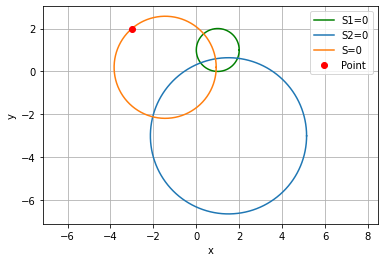
\includegraphics[width=\columnwidth]{solutions/4/4/3/figures/circles.png}
\caption{Plot of circles}
\label{4/4/3/fig:circles plot}
\end{figure}
